\documentclass{article}

\usepackage[dutch]{babel}
\usepackage[margin=3cm]{geometry}
\usepackage{graphicx}
\usepackage{float}
\usepackage{caption}
\usepackage{hyperref}
\usepackage{amsmath}
\usepackage{wrapfig}
\usepackage[parfill]{parskip}

% fonts
\usepackage[T1]{fontenc}
\usepackage{helvet}
\renewcommand{\familydefault}{\sfdefault}

\graphicspath{{img/}}
 
\newcommand{\bold}[1]{\textbf{#1}}

%Define the listing package
\usepackage{listings} %code highlighter
\usepackage{upquote}
\usepackage{color} %use color
\definecolor{mygreen}{rgb}{0,0.6,0}
\definecolor{mygray}{rgb}{0.5,0.5,0.5}
\definecolor{mymauve}{rgb}{0.58,0,0.82}

\begin{document}

\begin{titlepage}
    \author{Tuur Vanhoutte}
    \title{Security}
\end{titlepage}

\pagenumbering{gobble}
\maketitle
\newpage
\tableofcontents
\newpage

\pagenumbering{arabic}

\section{Security}

\subsection{Doel}
\begin{itemize}
    \item Security awareness  (bewustwording)
    \item Correcte nomenclatuur (communicatie)
    \item Advies over verantwoordelijkheden
    \item Inzien v/d consequenties v/h falen van security
    \item Situeren en herkennen van problemen
    \item Oplossingen correct implementeren
    \item Correcte methodieken toepassen
\end{itemize}

\subsection{Waarom?}

\begin{itemize}
    \item Niet iedereen heeft even goede bedoelingen
    \item Grote hoeveelheid mensen = veel potenti"ele slachtoffers (internet == iedereen zeer bereikbaar)
    \item Er is geen magische one-size-fits-all oplossing
    \item Verantwoordelijkheid van iedereen
    \item Tegenmaatregelen nemen
    \item Alert en voorzichtig zijn
\end{itemize}


\subsection{Tegenmaatregelen}
\begin{itemize}
    \item Zijn slechts nuttig indien ze effectief worden gebruikt
    \item Lijken vaak in de weg te zitten of lastig, maar zijn noodzakelijk
\end{itemize}

\subsection{Risico}

\begin{figure}[H]
    \centering
    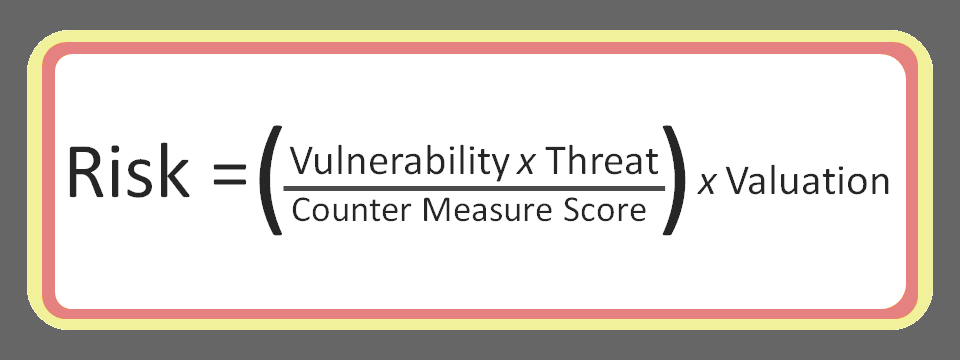
\includegraphics[width=0.4\textwidth]{risk.png}
    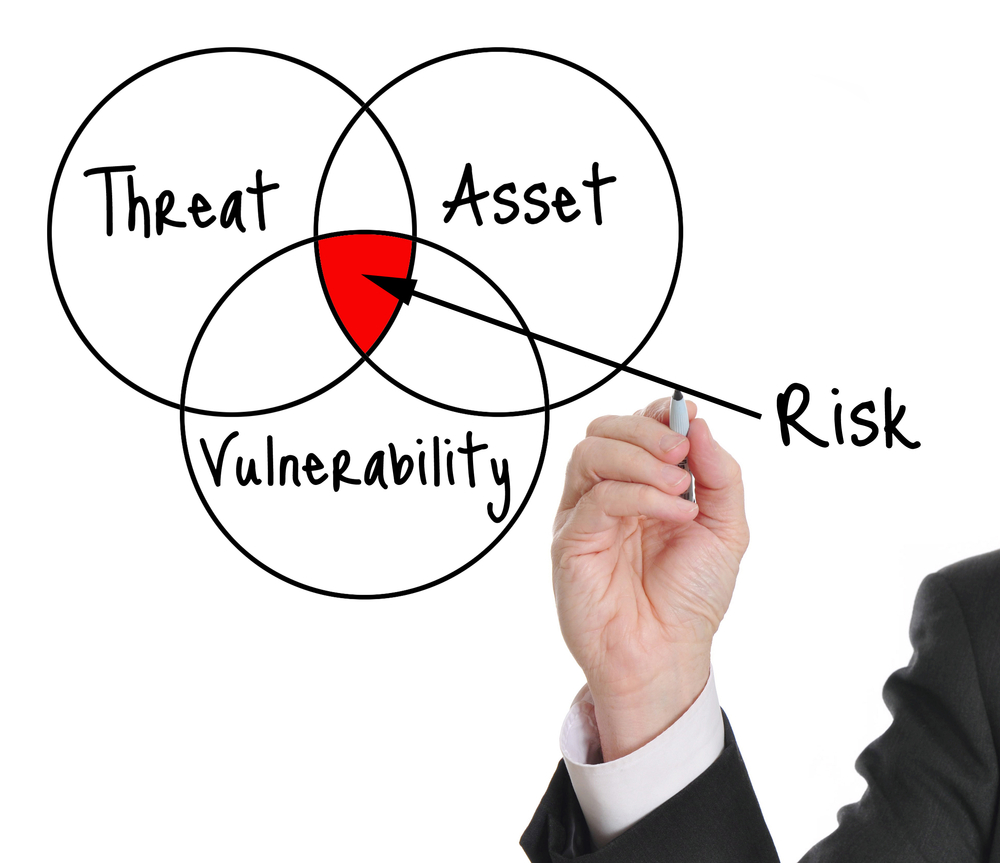
\includegraphics[width=0.25\textwidth]{01.png}
    \caption{Risico}
\end{figure}


\begin{itemize}
    \item De mate van bedreiging is niet beheersbaar
    \item De kwetsbaarheid is te reduceren door de implementatie van tegenmaatregelen
    \item Tegenmaatregelen reduceren kwetsbaarheid
    \item Bedrijfsimpact van het risico bepaalt de opportuniteit van de beveiligingsinvestering
    \item Bepalen van de financiële impact van een incident is uitermate bedrijfsspecifiek
\end{itemize}




\subsection{Theoretisch model}
\textcolor{red}{\bold{WORDT GEVRAAGD OP EXAMEN}}

\bold{CIA-model}

\begin{itemize}
    \item Confidentiality (Vertrouwelijkheid)
    \item Integrity (Integriteit)
    \item Availability (Beschikbaarheid)
\end{itemize}

\begin{figure}[H]
    \centering
    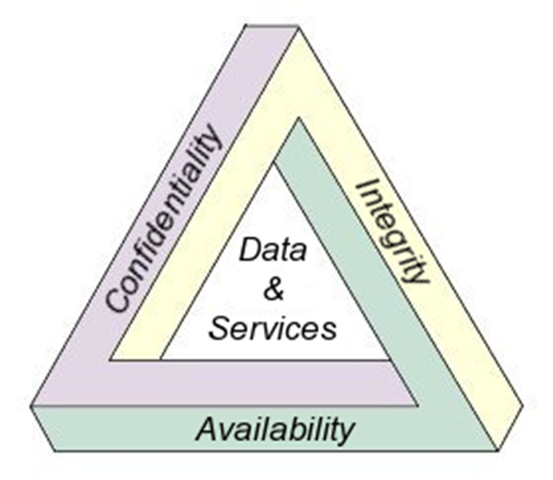
\includegraphics[width=0.3\textwidth]{cia-model.png}
    \caption{CIA-model}
\end{figure}

\bold{Vertrouwelijkheid}: gegevens kunnen \textit{enkel} door de juiste partijen worden geraadpleegd.

\bold{Integriteit}: gegevens zijn vaststaand en veranderen niet, tenzij de juiste, gemachtigde personen ze veranderen.

\bold{Beschikbaarheid}: de gegevens zijn beschikbaar en te bekijken door de juiste partijen, ongeacht aanvallen zoals DDOS-attacks.

\url{https://en.wikipedia.org/wiki/Information_security#Confidentiality}

\url{https://en.wikipedia.org/wiki/Information_security#Integrity}

\url{https://en.wikipedia.org/wiki/Information_security#Availability}

\subsection{Bedreiging vs kwetsbaarheid}
Bedreiging (threat)

Kwetsbaarheid (vulnerability)


\subsubsection{Bedreigde doelen}
\begin{itemize}
    \item Infrastructuur
    \item Gegevens
    \item Operationaliteit
\end{itemize}

\begin{figure}[H]
    \centering
    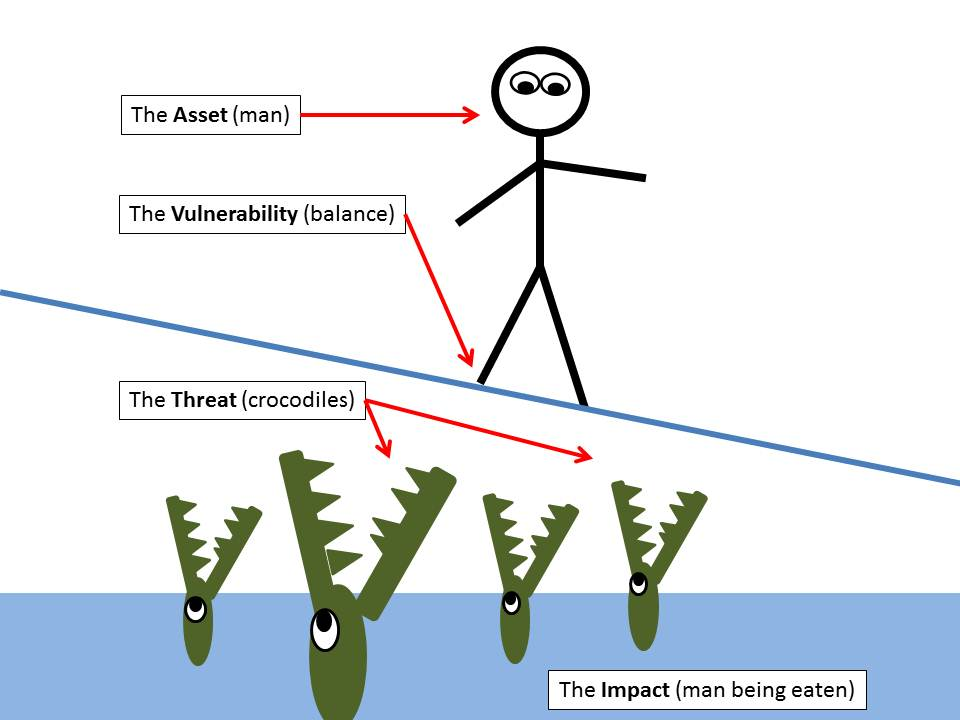
\includegraphics[width=0.5\textwidth]{crocodiles.jpg}
    \caption{}
\end{figure}



\end{document}